%%%%%%%%%%%%%%%%%%%%%%%%%%%%%%%%%%%%
% Slide options
%%%%%%%%%%%%%%%%%%%%%%%%%%%%%%%%%%%%

% Option 1: Slides with solutions

\documentclass[slidestop,compress,mathserif]{beamer}
\usepackage{booktabs}
\newcommand{\soln}[1]{\textit{#1}}
\newcommand{\solnGr}[1]{#1}

% Option 2: Handouts without solutions

%\documentclass[11pt,containsverbatim,handout]{beamer}
%\usepackage{booktabs}
%\usepackage{pgfpages}
%\pgfpagesuselayout{4 on 1}[letterpaper,landscape,border shrink=5mm]
%\newcommand{\soln}[1]{ }
%\newcommand{\solnGr}{ }

%%%%%%%%%%%%%%%%%%%%%%%%%%%%%%%%%%%%
% Style
%%%%%%%%%%%%%%%%%%%%%%%%%%%%%%%%%%%%
%%%%%%%%%%%%%%%%%%%%%%%%%%%%%%%%%%%%%%%%%%%%%%%%%%%%%%%%%%%%%%%%%%%%%%%%
% MA213/214 shared slide style
%
% "Calm & Cool" palette + content-type callout boxes.
% Overhauled (2026) from the original OpenIntro/metropolis style:
%   - all OpenIntro visual branding removed (logo, grid, colors)
%   - a low-key cool palette (see colors below)
%   - tcolorbox callout boxes so students recognize content types
% See common/README.md for the command cheat-sheet.
%%%%%%%%%%%%%%%%%%%%%%%%%%%%%%%%%%%%%%%%%%%%%%%%%%%%%%%%%%%%%%%%%%%%%%%%

\usetheme{metropolis}

%%%%%%%%%%%%%%%%
% Packages
%%%%%%%%%%%%%%%%

\usepackage{geometry}
\usepackage{graphicx}
\usepackage{amssymb}
\usepackage{epstopdf}
\usepackage{amsmath}  	% this permits text in eqnarray among other benefits
\usepackage{url}		% produces hyperlinks
\usepackage{hyperref}	% allows for color usage in tables
\usepackage[english]{babel}
\usepackage[latin1]{inputenc}
\usepackage{colortbl}	% allows for color usage in tables
\usepackage{multirow}	% allows for rows that span multiple rows in tables
\usepackage{color}		% this package has a variety of color options
\usepackage{pgf}
\usepackage{calc}
\usepackage{ulem}
\usepackage{multicol}
\usepackage{textcomp}
\usepackage{txfonts}
\usepackage{listings}
\usepackage{tikz}
\usepackage{array}
\usepackage{wasysym}
\usepackage{fancyvrb}
\usepackage{etoolbox}             % \ifstrempty for optional box subtitles
\usepackage[most]{tcolorbox}      % content-type callout boxes
\tcbuselibrary{listings}          % R-code block (\begin{rblock})
\usepackage{fontawesome5}         % box icons

%%%%%%%%%%%%%%%%
% Remove navigation symbols
%%%%%%%%%%%%%%%%

\setbeamertemplate{navigation symbols}{}

%%%%%%%%%%%%%%%%
% "Calm & Cool" palette
%%%%%%%%%%%%%%%%

% chrome / structure / body
\definecolor{ccSlate}{HTML}{2E3742}   % frametitle bar, structure, section pages (deep neutral slate)
\definecolor{ccInk}{HTML}{2B2B2B}     % body text
\definecolor{ccWash}{HTML}{FCF8F1}    % gentle warm title-slide background wash (complements the cool blues)

% example (blue)
\definecolor{ccBlue}{HTML}{2F6690}
\definecolor{ccBlueBg}{HTML}{EAF1F7}
% interactive activity / discussion (green)
\definecolor{ccGreen}{HTML}{4E8A6B}
\definecolor{ccGreenBg}{HTML}{E9F3EC}
% solution (purple)
\definecolor{ccPurple}{HTML}{6F5499}
\definecolor{ccPurpleBg}{HTML}{EFEAF6}
% worksheet / focused work (terracotta)
\definecolor{ccTerra}{HTML}{C2693E}
\definecolor{ccTerraBg}{HTML}{FAEDE4}
% formula / definition (neutral slate)
\definecolor{ccGray}{HTML}{5C6B7A}
\definecolor{ccGrayBg}{HTML}{EEF1F4}
% caution / common pitfall (brick red)
\definecolor{ccRed}{HTML}{B23A48}
\definecolor{ccRedBg}{HTML}{FAEAEC}
% key idea / takeaway (muted gold)
\definecolor{ccGold}{HTML}{9C7A28}
\definecolor{ccGoldBg}{HTML}{F7F1DF}
% learning goals / lesson outcomes (teal)
\definecolor{ccTeal}{HTML}{2C6E6B}
\definecolor{ccTealBg}{HTML}{E6F0EF}
% learning objectives (indigo)
\definecolor{ccIndigo}{HTML}{45507A}
\definecolor{ccIndigoBg}{HTML}{ECEEF4}
% R code / output (gray)
\definecolor{ccCode}{HTML}{5F5E5A}
\definecolor{ccCodeBg}{HTML}{F4F5F6}

% neutral grays kept from the original style
\definecolor{gray}{rgb}{0.5, 0.5, 0.5}
\definecolor{darkGray}{rgb}{0.3, 0.3, 0.3}
\definecolor{darkerGray}{rgb}{0.2, 0.2, 0.2}

% Backwards-compatible aliases: old OpenIntro color names now point at the
% new palette, so existing \textcolor{oiB}{...}, \hl{...}, etc. keep working.
\colorlet{oiB}{ccBlue}
\colorlet{oiG}{ccGreen}
\colorlet{hlblue}{ccBlue}
\colorlet{rubineRed}{ccRed}
\colorlet{irishGreen}{ccGreen}
\colorlet{lightGreen}{ccGreen}

%%%%%%%%%%%%%%%%
% Restyle metropolis with the Calm & Cool chrome
%%%%%%%%%%%%%%%%

\metroset{block=fill}

\setbeamercolor{normal text}{fg=ccInk, bg=white}
\setbeamercolor{structure}{fg=ccSlate}
\setbeamercolor{alerted text}{fg=ccBlue}
\setbeamercolor{example text}{fg=ccGreen}
\setbeamercolor{frametitle}{bg=ccSlate, fg=white}
\setbeamercolor{progress bar}{fg=ccBlue}
\setbeamercolor{title separator}{fg=ccBlue}
\setbeamercolor{title}{fg=ccSlate}
\setbeamercolor{subtitle}{fg=ccBlue}
\setbeamercolor{author}{fg=ccInk}
\setbeamercolor{institute}{fg=ccGray}
\setbeamercolor{date}{fg=ccGray}
\setbeamercolor{section title}{fg=ccSlate}
\setbeamercolor{standout}{fg=white, bg=ccSlate}

% Section pages sit on the same warm wash as the title slide. We keep
% metropolis's section-title styling and just paint a full-page ccWash
% background behind it (needs >=2 pdflatex passes for the current-page node).
\setbeamertemplate{section page}{%
  \begin{tikzpicture}[remember picture, overlay]
    \fill[ccWash] (current page.south west) rectangle (current page.north east);
  \end{tikzpicture}%
  \centering
  \begin{minipage}{22em}
    \raggedright
    \usebeamercolor[fg]{section title}%
    \usebeamerfont{section title}%
    \insertsectionhead\\[-1ex]
    \usebeamertemplate*{progress bar in section page}%
    \par
  \end{minipage}\par
  \vspace{\baselineskip}
}

%%%%%%%%%%%%%%%%
% Custom inline text commands (recolored to the palette)
%%%%%%%%%%%%%%%%

% degree
\newcommand{\degree}{\ensuremath{^\circ}}

% cite
\newcommand{\ct}[1]{
\vfill
{\tiny #1}}

\newcommand{\NamedNote}[2]{
\rule{2.5cm}{0.25pt} \\ \textit{\footnotesize{\textcolor{rubineRed}{#1:} \textcolor{darkerGray}{#2}}}}

% Note
\newcommand{\Note}[1]{
\rule{2.5cm}{0.25pt} \\ \textit{\footnotesize{\textcolor{rubineRed}{Note:} \textcolor{darkerGray}{#1}}}}

% Remember
\newcommand{\Remember}[1]{\textit{\scriptsize{\textcolor{ccTerra}{Remember:} #1}}}

% expected counts
\newcommand{\ex}[1]{\textit{\textcolor{ccBlue}{#1}}}

% red
\newcommand{\red}[1]{\textit{\textcolor{rubineRed}{#1}}}

% pink
\newcommand{\pink}[1]{\textit{\textcolor{rubineRed!90!white!50}{#1}}}

% green
\newcommand{\green}[1]{\textit{\textcolor{irishGreen}{#1}}}

% orange
\newcommand{\orange}[1]{\textit{\textcolor{ccTerra}{#1}}}

% links: webURL, webLink, appLink
\newcommand{\webURL}[1]{\urlstyle{same}{ \textit{\textcolor{darkGray}{\url{#1}}}}}
\newcommand{\webLink}[2]{\href{#1}{\textcolor{darkGray}{{#2}}}}
\newcommand{\appLink}[2]{\href{#1}{\textcolor{white}{{#2}}}}

% mail
\newcommand{\mail}[1]{\href{mailto:#1}{\textit{\textcolor{darkGray}{#1}}}}

% highlighting: hl, hlGr, mathhl
\newcommand{\hl}[1]{\textit{\textcolor{hlblue}{#1}}}
\newcommand{\hlGr}[1]{\textit{\textcolor{lightGreen}{#1}}}
\newcommand{\mathhl}[1]{\textcolor{hlblue}{\ensuremath{#1}}}

%%%%%%%%%%%%%%%%
% Structural helpers (unchanged from the original)
%%%%%%%%%%%%%%%%

% two col: two columns
\newenvironment{twocol}[4]{
\begin{columns}[c]
\column{#1\textwidth}
#3
\column{#2\textwidth}
#4
\end{columns}
}

% slot (for probability calculations)
\newenvironment{slot}[2]{
\begin{array}{c}
\underline{#1} \\
#2
\end{array}
}

% pr: left and right parentheses
\newcommand{\pr}[1]{
\left( #1 \right)
}

% cancel
\newcommand{\cancel}[1]{%
    \tikz[baseline=(tocancel.base)]{
        \node[inner sep=0pt,outer sep=0pt] (tocancel) {#1};
        \draw[red, line width=0.5mm] (tocancel.south west) -- (tocancel.north east);
    }%
}

% removepagenumbers
\newcommand{\removepagenumbers}{%
  \setbeamertemplate{footline}{}
}

% change margin
\newenvironment{changemargin}[2]{%
\begin{list}{}{%
\setlength{\topsep}{0pt}%
\setlength{\leftmargin}{#1}%
\setlength{\rightmargin}{#2}%
\setlength{\listparindent}{\parindent}%
\setlength{\itemindent}{\parindent}%
\setlength{\parsep}{\parskip}%
}%
\item}{\end{list}}

% footnote
\long\def\symbolfootnote[#1]#2{\begingroup%
\def\thefootnote{\fnsymbol{footnote}}\footnote[#1]{#2}\endgroup}

% commands from the book
\newenvironment{data}[1]{\texttt{#1}}{}
\newenvironment{var}[1]{\texttt{#1}}{}
\newenvironment{resp}[1]{\texttt{#1}}{}

%%%%%%%%%%%%%%%%
% Content-type callout boxes (tcolorbox)
%
% Each type has a colored title strip (icon + label) over a light fill.
% Color = content type; the label + icon reinforce it (so the cue does
% not rely on color alone).
%%%%%%%%%%%%%%%%

\tcbset{
  cccallout/.style 2 args={
    enhanced, breakable=false,
    colback=#2, colframe=#1, colbacktitle=#1, coltitle=white,
    fonttitle=\bfseries\footnotesize,
    boxrule=0.6pt, arc=2.5pt, outer arc=2.5pt,
    left=5pt, right=5pt, top=3pt, bottom=3pt, boxsep=2pt,
    toptitle=2pt, bottomtitle=2pt, lefttitle=5pt,
    before skip=5pt, after skip=5pt,
  },
}

% One-off / collection of examples (blue): \workedexample[subtitle]{body}.
% (Named \workedexample, not \example, because beamer defines \example.)
\newtcolorbox{examplebox}[1][]{cccallout={ccBlue}{ccBlueBg},
  title={\faIcon{lightbulb}~~Example\ifstrempty{#1}{}{ \textmd{---}\ #1}}}
\newcommand{\workedexample}[2][]{\begin{examplebox}[#1]#2\end{examplebox}}

% Running-example header (blue): \examplehead{name} at the top of each frame of a
% multi-slide running example. A one-off or a collection of examples uses the
% \workedexample box above instead.
\newcommand{\examplehead}[1]{%
  \vspace{-0.4em}\par\noindent\tcbox[on line, colback=ccBlue, colframe=ccBlue, coltext=white,
    boxrule=0pt, arc=2pt, left=5pt, right=5pt, top=1pt, bottom=1pt,
    box align=base, nobeforeafter]{\footnotesize\bfseries\faIcon{lightbulb}\,Running example}%
  \ifstrempty{#1}{}{\enspace{\footnotesize\bfseries\textcolor{ccBlue}{#1}}}%
  \par\nobreak\vspace{-0.6em}{\color{ccBlue}\rule{\linewidth}{0.7pt}}\par\nobreak\vspace{-0.8em}}

% Interactive activity (green): \activity[subtitle]{body}
\newtcolorbox{activitybox}[1][]{cccallout={ccGreen}{ccGreenBg},
  title={\faIcon{users}~~Activity\ifstrempty{#1}{}{ #1}}}
\newcommand{\activity}[2][]{\begin{activitybox}[#1]#2\end{activitybox}}

% Discussion question (green): \dq{body}
\newtcolorbox{dqbox}{cccallout={ccGreen}{ccGreenBg}, title={\faIcon{comments}~~Discussion}}
\newcommand{\dq}[1]{\begin{dqbox}#1\end{dqbox}}

% Solution (purple): \solnbox{body}. Gated by the per-deck \soln toggle, so it
% shows in the instructor build and vanishes from the student handout build.
% (Named \solnbox, not \solution, because beamer already defines \solution.)
\newtcolorbox{solutionbox}{cccallout={ccPurple}{ccPurpleBg}, title={\faIcon{key}~~Solution}}
\newcommand{\solnbox}[1]{\soln{\begin{solutionbox}#1\end{solutionbox}}}

% Worksheet / focused work (terracotta): \worksheet[subtitle]{body}
\newtcolorbox{worksheetbox}[1][]{cccallout={ccTerra}{ccTerraBg},
  title={\faIcon{pencil-alt}~~Worksheet\ifstrempty{#1}{}{ #1}}}
\newcommand{\worksheet}[2][]{\begin{worksheetbox}[#1]#2\end{worksheetbox}}

% Formula / definition (neutral slate). Supports both real usages found in the
% decks: \formula{title}{body} and the bare \formula{body} (title defaults to
% "Formula"). The second group is an optional brace argument.
\newtcolorbox{formulabox}[1][Formula]{cccallout={ccGray}{ccGrayBg},
  title={\faIcon{square-root-alt}~~#1}}
\NewDocumentCommand{\formula}{m g}{%
  \IfNoValueTF{#2}%
    {\begin{formulabox}#1\end{formulabox}}%
    {\begin{formulabox}[#1]#2\end{formulabox}}}

% Common pitfall / caution (brick red): \caution[subtitle]{body}
\newtcolorbox{cautionbox}[1][]{cccallout={ccRed}{ccRedBg},
  title={\faIcon{exclamation-triangle}~~Caution\ifstrempty{#1}{}{ #1}}}
\newcommand{\caution}[2][]{\begin{cautionbox}[#1]#2\end{cautionbox}}

% Key idea / takeaway (muted gold): \keyidea[subtitle]{body}
\newtcolorbox{keyideabox}[1][]{cccallout={ccGold}{ccGoldBg},
  title={\faIcon{star}~~Key idea\ifstrempty{#1}{}{ #1}}}
\newcommand{\keyidea}[2][]{\begin{keyideabox}[#1]#2\end{keyideabox}}

% Learning goals / lesson outcomes (teal): \goals{body}. Sits under the short
% LO headings on the objectives slide; body is the "you should be able to" list.
\newtcolorbox{goalsbox}{cccallout={ccTeal}{ccTealBg}, fontupper=\footnotesize,
  top=1pt, bottom=2pt, boxsep=1pt, before skip=3pt,
  title={\faIcon{bullseye}~~By the end of today, you should be able to\ldots}}
\newcommand{\goals}[1]{\begin{goalsbox}#1\end{goalsbox}}

% Learning objectives (indigo): \objectives{body} -- the formal LO headings,
% shown alongside \goals on the objectives slide.
\newtcolorbox{objectivesbox}{cccallout={ccIndigo}{ccIndigoBg}, fontupper=\small,
  top=1pt, bottom=2pt, boxsep=1pt, before skip=3pt,
  title={\faIcon{clipboard-list}~~Learning objectives}}
\newcommand{\objectives}[1]{\begin{objectivesbox}#1\end{objectivesbox}}

% Defaults for a bare \begin{lstlisting}. Without these it inherits the listings
% package defaults: 11pt type, fixed-width columns (which spaces code out as
% "a g e _ f i t"), and no line breaking, so a long line silently runs off the
% right edge of the slide. A deck that passes its own basicstyle still wins.
% Layout only -- syntax coloring is left to the \begin{rblock} environment.
\lstset{
  basicstyle=\ttfamily\footnotesize, columns=fullflexible,
  breaklines=true, breakindent=1.5em, showstringspaces=false,
  numbers=none, frame=none}

% R code / output (gray): \begin{rblock}[subtitle] ... \end{rblock}
% NOTE: a frame containing an rblock must be declared \begin{frame}[fragile].
\lstdefinestyle{ccR}{
  language=R, basicstyle=\ttfamily\footnotesize, columns=fullflexible,
  breaklines=true, showstringspaces=false, numbers=none, frame=none,
  keywordstyle=\color{ccBlue}, commentstyle=\color{ccGreen!75!black},
  stringstyle=\color{ccTerra}}
\newtcblisting{rblock}[1][]{cccallout={ccCode}{ccCodeBg},
  title={\faIcon{terminal}~~R\ifstrempty{#1}{}{ #1}},
  listing only, listing style=ccR}

% --- Legacy boxes (kept so existing decks compile) ---

% app: application exercise -> alias of activity
\newcommand{\app}[1]{\activity{#1}}

% pq: practice question (green, interactive family)
\newtcolorbox{pqbox}{cccallout={ccGreen}{ccGreenBg}, title={\faIcon{list-ol}~~Practice}}
\newcommand{\pq}[1]{\begin{pqbox}#1\end{pqbox}}

% solnMult: solutions for multiple-choice practice questions (uses \soln toggle)
\newcommand{\solnMult}[1]{
\item[] \vspace{-0.59cm}
\only<1>{\item #1}
\soln{\only<2->{\item \orange{#1}}}
}

%%%%%%%%%%%%%%%%
% De-branded title frame + attribution
%%%%%%%%%%%%%%%%

% Eyebrow line on the title slide; a deck may \renewcommand this.
\newcommand{\coursetag}{MA214: Applied Statistics}

% Attribution: all slides released under CC BY-SA, crediting both the
% instructor (later material) and OpenIntro (basis of the earlier material).
\newcommand{\courseattribution}{%
  Slides by Jonathan H.~Huggins, building on materials from OpenIntro's
  \emph{Introduction to Modern Statistics} (Mine \c{C}etinkaya-Rundel et al.).
  Released under the
  \webLink{http://creativecommons.org/licenses/by-sa/3.0/us/}{CC BY-SA license}.
  Some images included under fair use (educational purposes).}

% \maketitleframe: de-branded title slide (no logo, no grid). Uses the deck's
% \title, \subtitle, and \coursetag.
\newcommand{\maketitleframe}{%
  \addtocounter{framenumber}{-1}%
  {\removepagenumbers
  \setbeamercolor{background canvas}{bg=ccWash}%
  \begin{frame}[plain]
    \vspace*{2.6em}
    {\color{ccSlate}\rule{\textwidth}{2.5pt}}\par\vspace{1.5em}
    {\usebeamerfont{date}\scshape\color{ccGray}\coursetag}\par\vspace{0.55em}
    {\usebeamerfont{title}\color{ccSlate}\inserttitle\par}
    \vspace{0.45em}{\color{ccBlue}\rule{3em}{2.5pt}}\par\vspace{0.7em}
    {\usebeamerfont{subtitle}\color{ccBlue}\insertsubtitle\par}
    \vfill
    {\color{ccGray!55}\rule{\textwidth}{0.4pt}}\par\vspace{0.45em}
    {\tiny\color{ccGray}\courseattribution\par}
    \vspace*{0.4em}
  \end{frame}}}

%%%%%%%%%%%%%%%%
% Graphics
%%%%%%%%%%%%%%%%

\DeclareGraphicsRule{.tif}{png}{.png}{`convert #1 `dirname #1`/`basename #1 .tif`.png}

\graphicspath{ {../../common/} {figures/} }

% Preamble
\title[Lecture 19]{Lecture 19: Posterior approximation}
\subtitle{Module 4: Bayesian Statistics}
\author{Jonathan H.~Huggins}
\institute{}
\date{}

\begin{document}

%%%%%%%%%%%%%%%%%%%%%%%%%%%%%%%%%%%%
% Title page
%%%%%%%%%%%%%%%%%%%%%%%%%%%%%%%%%%%%

\maketitleframe

%%%%%%%%%%%%%%%%%%%%%%%%%%%%%%%%%%%%
% Agenda
%%%%%%%%%%%%%%%%%%%%%%%%%%%%%%%%%%%%
% !TEX root =  Lecture19.tex


%%%%%%%%%%%%%%%%%%%%%%%%%%%%%%%%%%%%
% Recap/Agenda
%%%%%%%%%%%%%%%%%%%%%%%%%%%%%%%%%%%%
\begin{frame}
\frametitle{Module 4: Bayesian Statistics}
    \begin{itemize}
        \item \hl{Previously:} conjugate models: the posterior in closed form, its mean a weighted average of prior and data.
        \item \hl{This time:} what to do when there is \emph{no} closed form (the usual case), so we must \hl{approximate} the posterior.
          \begin{itemize}
              \item why the normalizing constant is the obstacle;
              \item \hl{grid approximation}, turning the integral into a sum;
              \item \hl{Markov chain Monte Carlo}, sampling from the posterior instead;
              \item reading the output: \hl{trace plots}, burn-in, step size, diagnostics.
          \end{itemize}
        \item \hl{Reading:} Bayes Rules!\ Chapters 6 and 7.
        \item \hl{Homework:}
    \end{itemize}
\end{frame}


%%%%%%%%%%%%%%%%%%%%%%%%%%%%%%%%%%%%
% Learning objectives:
%%%%%%%%%%%%%%%%%%%%%%%%%%%%%%%%%%%%
\begin{frame}
    \frametitle{Lecture Objectives}
    \goals{%
    \begin{itemize}
    \item explain why a non-conjugate model has \hl{no closed-form posterior}, and identify the normalizing constant as the obstacle;
    \item use \hl{grid approximation} to turn the posterior integral into a sum, and say why it breaks down as the number of parameters grows;
    \item describe how \hl{Metropolis--Hastings} MCMC draws posterior samples via propose / accept-or-reject, and read an \hl{acceptance probability};
    \item diagnose a chain from its \hl{trace plot}: estimate the \hl{burn-in}, spot a \hl{step size} that is too large or too small;
    \item say what \hl{R-hat}, \hl{ESS}, and \hl{MCSE} each tell you about whether to trust the output.
    \end{itemize}}
\end{frame}


%%%%%%%%%%%%%%%%%%%%%%%%%%%%%%%%%%%%
\begin{frame}
    \frametitle{Lecture Objectives}
    \objectives{%
    \begin{itemize}
    \item \textbf{(M4, LO5)} Using Markov chain Monte Carlo
    \end{itemize}}
    \vspace{0.3em}
    {\small Building on, and revisiting:}
    \objectives{%
    \begin{itemize}
    \item \textbf{(M4, LO3)} Conjugate Models: the whale-sightings posterior from Lecture 18, now recomputed \emph{without} conjugacy
    \end{itemize}}
\end{frame}


%%%%%%%%%%%%%%%%%%%%%%%%%%%%%%%%%%%%
% Section: When Conjugacy Fails
%%%%%%%%%%%%%%%%%%%%%%%%%%%%%%%%%%%%
\section{When conjugacy fails}

\begin{frame}
\frametitle{The limits of conjugate priors}

Lecture 18 gave three \hl{conjugate families}:
\begin{itemize}
    \item Beta prior $+$ Binomial likelihood $\Rightarrow$ Beta posterior
    \item Normal prior $+$ Normal likelihood $\Rightarrow$ Normal posterior
    \item Gamma prior $+$ Poisson likelihood $\Rightarrow$ Gamma posterior
\end{itemize}

\pause
\medskip

\hl{But conjugate priors are the exception, not the rule:}
\begin{itemize}
    \item our prior beliefs may not fit a conjugate family;
    \item the model may have several unknown parameters;
    \item the likelihood may admit no conjugate prior at all.
\end{itemize}

\pause
\medskip

\dq{What do we do when there's no closed-form posterior?}
\end{frame}

%%%%%%%%%%%%%%%%%%%%%%%%%%%%%%%%%%%%%%%%%%%%%%%%%%%%%%%%%%%%%%%%%%%%%%%%
\begin{frame}
\frametitle{A prior no conjugate family can match}

What if your genuine belief is \emph{bimodal}: a drug either mostly fails or mostly works, two camps of opinion?

\begin{center}
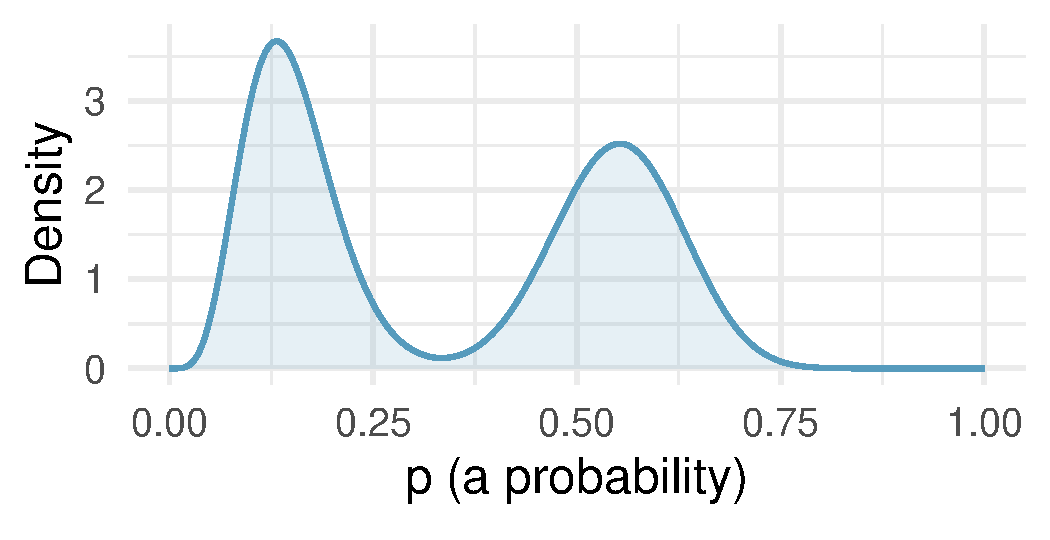
\includegraphics[width=0.66\textwidth]{bimodal_prior.pdf}
\end{center}

\vspace{-0.4em}
No $\text{Beta}(\alpha,\beta)$ has two humps. Forcing a conjugate prior here encodes what is \emph{convenient}, not what you believe.

\end{frame}

%%%%%%%%%%%%%%%%%%%%%%%%%%%%%%%%%%%%%%%%%%%%%%%%%%%%%%%%%%%%%%%%%%%%%%%%
\begin{frame}
\frametitle{The whale data, without conjugacy}

Whale sighting data from Lecture 18: $n = 7$ days, $\sum x_i = 31$, $\bar{x} = 4.43$

\medskip

\hl{Lecture 18:} $\text{Gamma}(6, 2)$ prior, conjugate to Poisson

\pause
\bigskip

\hl{But what if our prior beliefs don't match a Gamma shape?}

\pause
\medskip

\begin{itemize}
    \item Put the uncertainty on the \emph{log scale}: $\log(\lambda) \sim N(\log 3,\, 0.5^{2})$
    \item This gives a \hl{log-normal prior}: right-skewed, heavier tails than Gamma
    \item Log-normal is \emph{not} conjugate to Poisson, so there is no closed-form posterior
\end{itemize}
\end{frame}

%%%%%%%%%%%%%%%%%%%%%%%%%%%%%%%%%%%%%%%%%%%%%%%%%%%%%%%%%%%%%%%%%%%%
\begin{frame}[fragile]
\frametitle{Comparing Gamma and Log-Normal priors}
\examplehead{Whale sightings}

\begin{center}
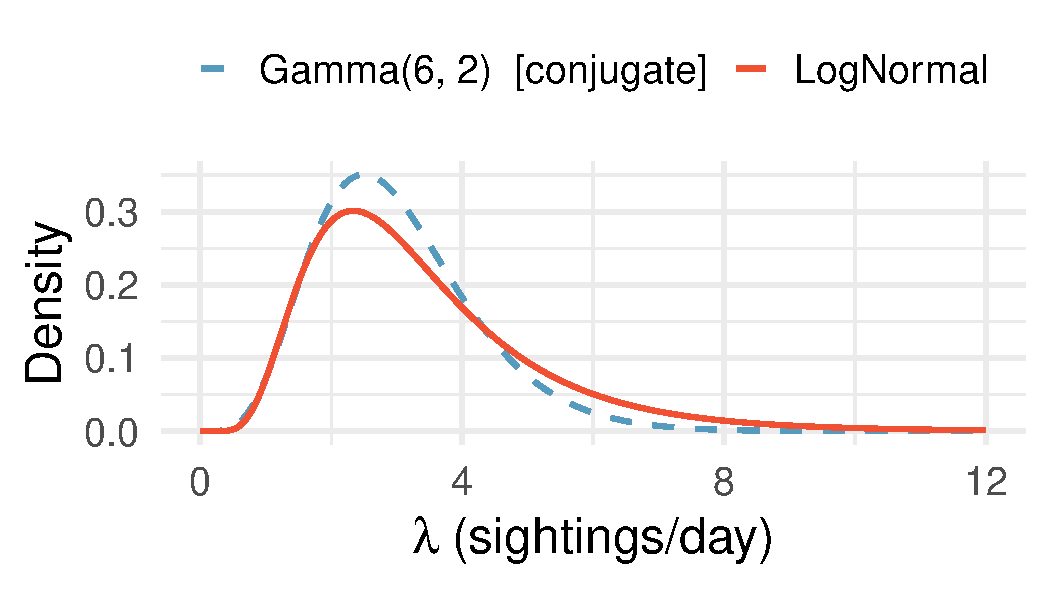
\includegraphics[width=0.85\textwidth]{lognormal_vs_gamma.pdf}
\end{center}

Both centered near $\lambda = 3$, but log-normal has heavier right tail.
\end{frame}

%%%%%%%%%%%%%%%%%%%%%%%%%%%%%%%%%%%%%%%%%%%%%%%%%%%%%%%%%%%%%%%%%%%%
\begin{frame}
\frametitle{The core problem}

Bayes' rule for random variables:
\[
f(\lambda \mid \mathbf{x}) = \frac{f(\lambda)\, L(\lambda\,; \mathbf{x})}{\displaystyle\int f(\lambda')\, L(\lambda'\,; \mathbf{x})\, d\lambda'}
\]
That $\int$ just means \emph{add up} prior $\times$ likelihood over \emph{every} $\lambda$.

\pause
\medskip

\begin{itemize}
    \item \hl{Numerator:} easy, just multiply prior $\times$ likelihood at any $\lambda$.
    \pause
    \item \hl{Denominator:} the hard part. For most models that sum has \emph{no formula}. Conjugacy let us skip it; otherwise we must \hl{approximate}.
\end{itemize}

\pause
\dq{If we cannot do the integral exactly, how might we get around it?}
\end{frame}

%%%%%%%%%%%%%%%%%%%%%%%%%%%%%%%%%%%%%%%%%%%%%%%%%%%%%%%%%%%%%%%%%%%%
\begin{frame}
\frametitle{Two computational strategies}

\begin{enumerate}
    \item \hl{Grid approximation:} Discretize parameter space, evaluate posterior on a grid
    \begin{itemize}
        \item Simple
        \item Works well in a \emph{few} dimensions (roughly 1--3)
    \end{itemize}
    \pause
    \medskip
    \item \hl{Markov Chain Monte Carlo (MCMC):} Draw \emph{samples} from the posterior via a random walk
    \begin{itemize}
        \item Scales to many dimensions
        \item The standard approach in practice
    \end{itemize}
\end{enumerate}

\end{frame}

%%%%%%%%%%%%%%%%%%%%%%%%%%%%%%%%%%%%
% Section: Grid Approximation
%%%%%%%%%%%%%%%%%%%%%%%%%%%%%%%%%%%%
\section{Grid approximation}

\begin{frame}
\frametitle{The idea: a discrete approximation}

\keyidea{Replace the continuous $\lambda$ with a finite grid $\lambda_1, \ldots, \lambda_K$. Evaluate prior $\times$ likelihood at each point, then normalize so the values sum to one. The intractable \emph{integral} has become a plain \emph{sum}.}

\pause
\medskip

Every quantity we want (mean, interval, tail probability) is then computed from $K$ numbers.
\end{frame}

%%%%%%%%%%%%%%%%%%%%%%%%%%%%%%%%%%%%%%%%%%%%%%%%%%%%%%%%%%%%%%%%%%%%
\begin{frame}[fragile]
\frametitle{Grid approximation, step by step}
\examplehead{Whale sightings}

\begin{center}
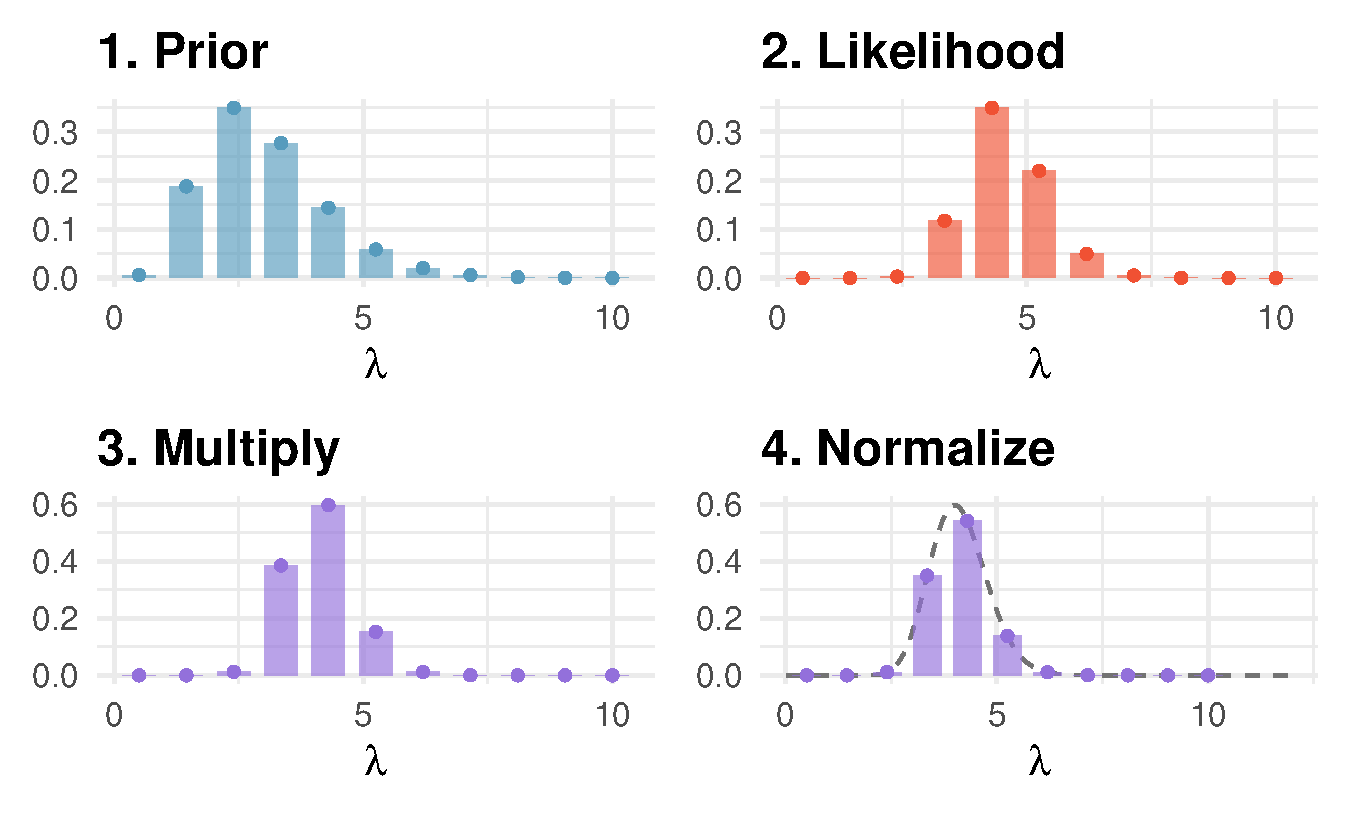
\includegraphics[width=0.90\textwidth]{grid_idea.pdf}
\end{center}
\end{frame}

%%%%%%%%%%%%%%%%%%%%%%%%%%%%%%%%%%%%%%%%%%%%%%%%%%%%%%%%%%%%%%%%%%%%
\begin{frame}
\frametitle{The 4-step grid approximation algorithm}

\begin{enumerate}
    \item \hl{Define the grid:} Choose grid points $\lambda_1, \ldots, \lambda_K$ spanning the support
    \medskip
    \item \hl{Evaluate:} Compute the un-normalized posterior
    \[
    g(\lambda_k) = f(\lambda_k) \cdot L(\lambda_k\,; \mathbf{x}) \quad \text{for each } k
    \]
    \medskip
    \item \hl{Normalize:} Divide by the sum to get posterior probabilities $q_k$
    \[
    q_k = \frac{g(\lambda_k)}{\sum_{j=1}^K g(\lambda_j)}
    \]
    \medskip
    \item \hl{Sample or summarize:} Treat $(\lambda_k, q_k)$ as a discrete distribution
\end{enumerate}
\end{frame}

%%%%%%%%%%%%%%%%%%%%%%%%%%%%%%%%%%%%%%%%%%%%%%%%%%%%%%%%%%%%%%%%%%%%
\begin{frame}
\frametitle{Computing summaries from the grid}

Grid approximation is $\hat P(\lambda = \lambda_{k} \mid \mathbf{x}) = q_{k}$

\hl{Posterior mean:}
\[
E(\lambda \mid \mathbf{x}) \;\approx\; \sum_{k=1}^K \lambda_k \, q_k \;=:\; \hat\lambda_{\text{grid}}
\]
\pause

\hl{Posterior variance:}
\[
\text{Var}(\lambda \mid \mathbf{x}) \;\approx\; \sum_{k=1}^K (\lambda_k - \hat\lambda_{\text{grid}})^2 \, q_k
\]
\pause

\end{frame}

%%%%%%%%%%%%%%%%%%%%%%%%%%%%%%%%%%%%%%%%%%%%%%%%%%%%%%%%%%%%%%%%%%%%
\begin{frame}
\frametitle{Intervals and probabilities from the grid}

\hl{95\% credible interval:} find $\lambda_a$ and $\lambda_b$ such that
\[
\sum_{k:\, \lambda_k \le \lambda_a} q_k = 0.025 \qquad \text{and} \qquad \sum_{k:\, \lambda_k \le \lambda_b} q_k = 0.975
\]
\pause
\hl{Posterior probability:} for any claim, add up the $q_k$ it covers. For the whales,
\[
P(\lambda > 3 \mid \mathbf{x}) = \sum_{k:\, \lambda_k > 3} q_k
\]
\pause
Means and probabilities are sums over the grid; the interval is a running total. No integration anywhere.

\end{frame}

%%%%%%%%%%%%%%%%%%%%%%%%%%%%%%%%%%%%%%%%%%%%%%%%%%%%%%%%%%%%%%%%%%%%
\begin{frame}[fragile]
\frametitle{Sanity check: how many grid points?}
\examplehead{Whale sightings}

The $\text{Gamma}(6, 2)$ prior gives a known posterior to check the grid against.

\begin{center}
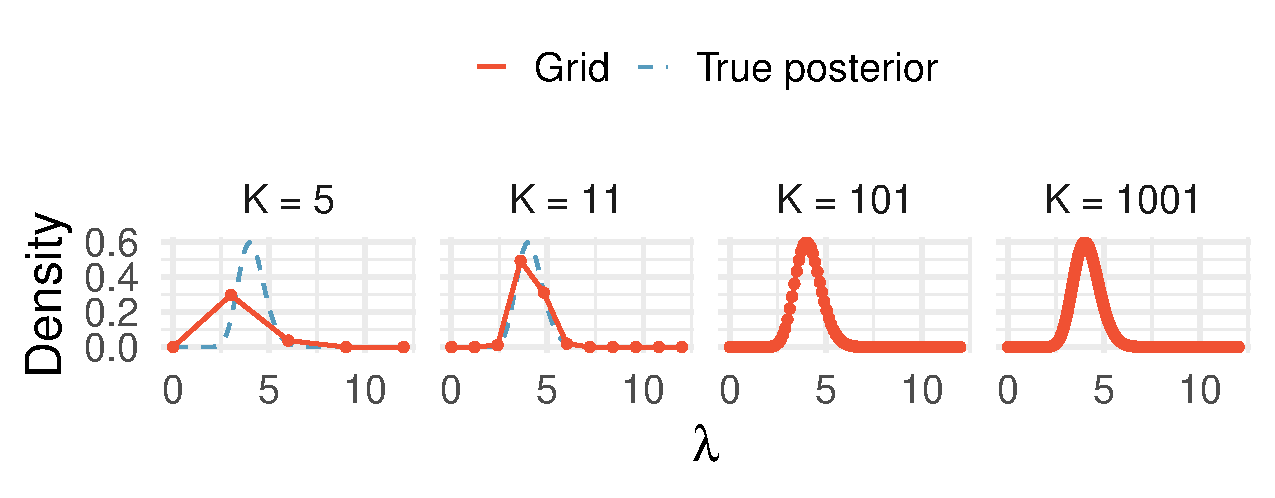
\includegraphics[width=0.90\textwidth]{grid_refinement_poisson.pdf}
\end{center}

A coarse grid cannot represent the shape. By $K = 101$ the approximation is indistinguishable from the truth.
\end{frame}

%%%%%%%%%%%%%%%%%%%%%%%%%%%%%%%%%%%%%%%%%%%%%%%%%%%%%%%%%%%%%%%%%%%%
\begin{frame}
\frametitle{Applying grid to the Log-Normal prior}
\examplehead{Whale sightings}

Log-normal prior, $n = 7$, $\sum x_i = 31$. Run the grid; compare against the conjugate Gamma:

\begin{center}
{\scriptsize
\renewcommand{\arraystretch}{1.0}
\begin{tabular}{l c c}
\toprule
& \textbf{Log-Normal prior} & \textbf{Gamma prior} \\
\midrule
Prior mean        & $3.40$         & $3.00$ \\
Prior 95\% CI      & $[1.1,\, 8.0]$  & $[1.1,\, 5.8]$ \\
\midrule
Posterior mean    & $4.24$         & $4.11$ \\
Posterior 95\% CI & $[2.9,\, 5.8]$  & $[2.9,\, 5.5]$ \\
$P(\lambda > 3 \mid \mathbf{x})$ & $0.97$ & $0.96$ \\
\bottomrule
\end{tabular}}
\end{center}

\pause
The \emph{priors} differ, yet the \emph{posteriors} nearly agree: 7 days of data outweigh the prior's shape. For the log-normal, only \hl{grid} could get us here.
\end{frame}

%%%%%%%%%%%%%%%%%%%%%%%%%%%%%%%%%%%%%%%%%%%%%%%%%%%%%%%%%%%%%%%%%%%%
\begin{frame}[fragile]
\frametitle{Comparing posteriors}
\examplehead{Whale sightings}

\begin{center}
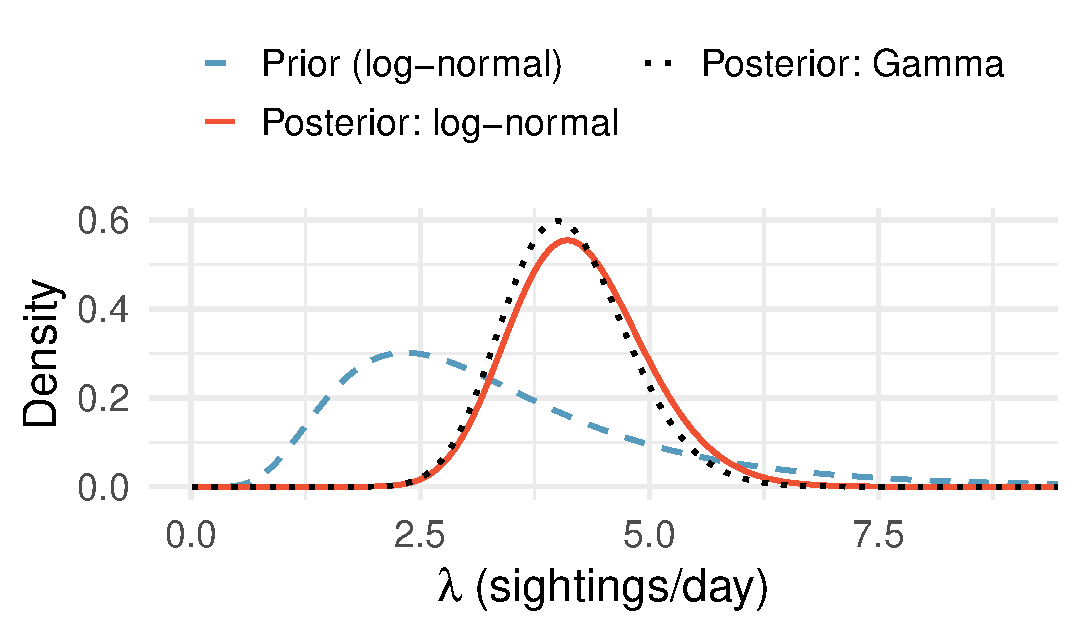
\includegraphics[width=0.85\textwidth]{lognormal_posterior.pdf}
\end{center}
\end{frame}

%%%%%%%%%%%%%%%%%%%%%%%%%%%%%%%%%%%%%%%%%%%%%%%%%%%%%%%%%%%%%%%%%%%%
\begin{frame}
\frametitle{Limitations of grid approximation}

\begin{itemize}
    \item \hl{Curse of dimensionality:} $K$ points/dimension $\Rightarrow$ $K^d$ total points

    \medskip
    \begin{center}
    \begin{tabular}{crl}
    \toprule
    \textbf{Dimensions ($d$)} & \textbf{Grid points ($K^d$)} & \textbf{Feasible?} \\
    \midrule
    1 & 100 & $\checkmark$ \\
    5 & 10,000,000,000 & ?? \\
    10 & $10^{20}$ & $\times$ \\
    \bottomrule
    \end{tabular}
    \end{center}
    \pause
    \medskip
    \item \hl{Grid bounds:} Must truncate unbounded parameter spaces
    \pause
    \item \hl{Not adaptive:} most of the grid sits where the posterior is near zero
    \pause
\end{itemize}
\caution{More adaptive grid schemes exist, but they still reach only about $d = 10$. Beyond that, grid approximation is not an option.}
\end{frame}

%%%%%%%%%%%%%%%%%%%%%%%%%%%%%%%%%%%%
% Section: Monte Carlo and MCMC
%%%%%%%%%%%%%%%%%%%%%%%%%%%%%%%%%%%%
\section{Monte Carlo sampling}

\begin{frame}
\frametitle{Sampling as a tool}

Three places sampling has already appeared:
\begin{itemize}
    \item \hl{Random sampling} from a population $\Rightarrow$ estimate population parameters
    \pause
    \item \hl{Permutation sampling} under $H_0$ $\Rightarrow$ approximate the null distribution
    \pause
    \item \hl{Bootstrap resampling} from the data $\Rightarrow$ approximate the sampling distribution
\end{itemize}

\pause
\medskip

\hl{Pattern:} draw many samples from a distribution, use them to approximate the properties we care about.

\pause
\medskip

\dq{What if we could sample from the posterior?}
\end{frame}

%%%%%%%%%%%%%%%%%%%%%%%%%%%%%%%%%%%%%%%%%%%%%%%%%%%%%%%%%%%%%%%%%%%%
\begin{frame}
\frametitle{Posterior summaries from samples}

If we have samples $\lambda^{(1)}, \ldots, \lambda^{(M)}$ from the posterior:

\pause
\medskip

\begin{itemize}
    \item Posterior mean $\approx$ sample mean of $\lambda^{(1)}, \ldots, \lambda^{(M)}$
    \item 95\% CI $\approx$ 2.5th and 97.5th percentiles
    \item $P(\lambda > 3 \mid \mathbf{x}) \approx$ fraction with $\lambda^{(m)} > 3$
\end{itemize}

\pause
\bigskip

This is \hl{Monte Carlo}: using random samples to summarize a distribution.

\pause
\bigskip

\dq{But how can we generate random samples from the posterior distribution?}
\end{frame}

%%%%%%%%%%%%%%%%%%%%%%%%%%%%%%%%%%%%%%%%%%%%%%%%%%%%%%%%%%%%%%%%%%%%
\begin{frame}
\frametitle{Markov Chain Monte Carlo (MCMC)}

\hl{MCMC:} a random walk through parameter space that produces posterior samples.

\pause
\medskip

The simplest version is \hl{Random Walk Metropolis--Hastings (RWMH)}:
\begin{enumerate}
    \item Start at some initial value $\lambda^{(0)}$
    \pause
    \medskip
    \item \hl{Propose} a new value: $\lambda^* = \lambda^{(m)} + \epsilon$, where $\epsilon \sim N(0, \text{step}^2)$
    \pause
    \medskip
    \item Compute the \hl{acceptance ratio}: $r = \dfrac{f(\lambda^* \mid \mathbf{x})}{f(\lambda^{(m)} \mid \mathbf{x})}$
    \pause
    \medskip
    \item \hl{Accept or reject}: if $r \geq 1$, move; if $r < 1$, move with probability $r$
    \pause
    \medskip
    \item Repeat steps 2--4
\end{enumerate}
\end{frame}

%%%%%%%%%%%%%%%%%%%%%%%%%%%%%%%%%%%%%%%%%%%%%%%%%%%%%%%%%%%%%%%%%%%%
\begin{frame}[fragile]
\frametitle{RWMH: an accepted step}
\examplehead{Whale sightings}

Using our log-normal posterior (non-conjugate, right-skewed):

\twocol{0.50}{0.50}{
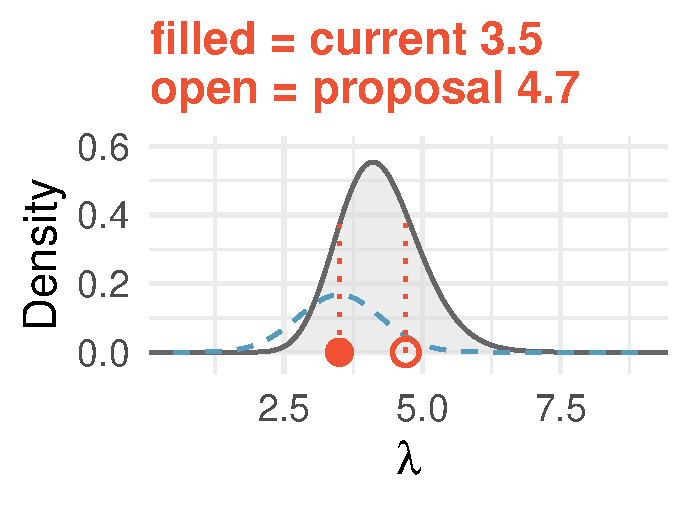
\includegraphics[width=\textwidth]{rwmh_propose_accept.pdf}
}{
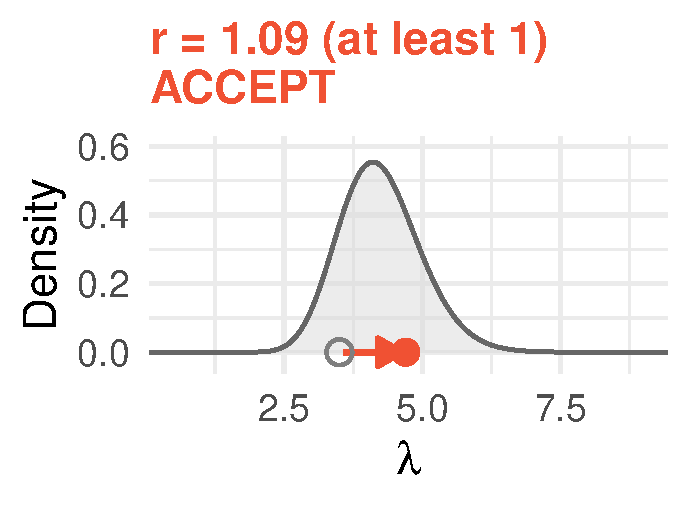
\includegraphics[width=\textwidth]{rwmh_accept.pdf}
}

$\lambda^* = 4.7$ has \emph{higher} posterior density than $\lambda^{(m)} = 3.5$, so $r \geq 1$ and the move is always accepted.
\end{frame}

%%%%%%%%%%%%%%%%%%%%%%%%%%%%%%%%%%%%%%%%%%%%%%%%%%%%%%%%%%%%%%%%%%%%
\begin{frame}[fragile]
\frametitle{RWMH: a rejected step}
\examplehead{Whale sightings}

\vspace{1.4em}

\twocol{0.50}{0.50}{
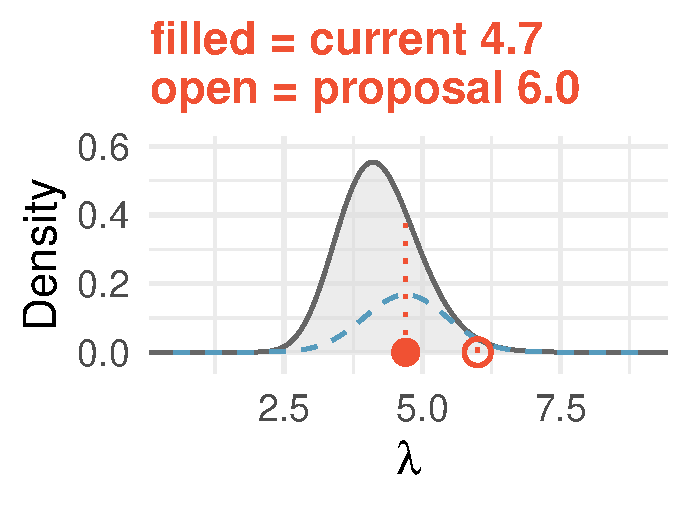
\includegraphics[width=\textwidth]{rwmh_propose_reject.pdf}
}{
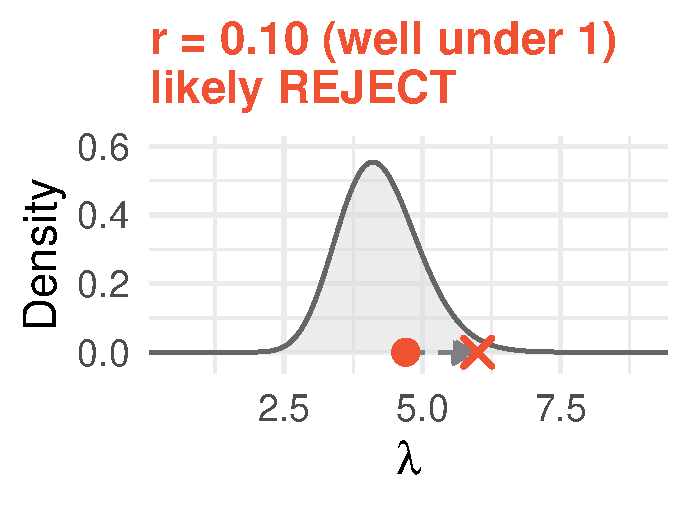
\includegraphics[width=\textwidth]{rwmh_reject.pdf}
}

$\lambda^* = 6.0$ has \emph{lower} density than $\lambda^{(m)} = 4.7$, so $r \ll 1$ and the proposal is likely rejected.
\end{frame}

%%%%%%%%%%%%%%%%%%%%%%%%%%%%%%%%%%%%%%%%%%%%%%%%%%%%%%%%%%%%%%%%%%%%
\begin{frame}
\frametitle{Why this works}

The chain spends more time in high-density regions:
\begin{itemize}
    \item proposals \emph{toward} the peak tend to be accepted;
    \item proposals \emph{away} from the peak tend to be rejected.
\end{itemize}

\pause
\bigskip

\keyidea{After enough steps, the \hl{fraction of time} the chain spends near each $\lambda$ is proportional to $f(\lambda \mid \mathbf{x})$, so the visited values \emph{are} a posterior sample.}

\end{frame}

%%%%%%%%%%%%%%%%%%%%%%%%%%%%%%%%%%%%%%%%%%%%%%%%%%%%%%%%%%%%%%%%%%%%%%%%
\begin{frame}
\frametitle{Tuning the step size}

The one knob is the proposal \hl{step size}, and the \hl{acceptance rate} (fraction of proposals accepted) tells you how it is set:

\medskip
\begin{itemize}
    \item \hl{Too small} $\Rightarrow$ almost everything accepted, but the chain barely moves;
    \pause
    \item \hl{Too large} $\Rightarrow$ almost everything rejected, the chain gets stuck;
    \pause
    \item \hl{Just right} $\Rightarrow$ acceptance around \hl{20--50\%}, and the chain explores efficiently.
\end{itemize}

\pause
\medskip

So the acceptance rate is a \hl{one-number health check}, available before you even look at a plot.
\end{frame}

%%%%%%%%%%%%%%%%%%%%%%%%%%%%%%%%%%%%%%%%%%%%%%%%%%%%%%%%%%%%%%%%%%%%
\begin{frame}[fragile]
\frametitle{Reading the trace plot: a healthy chain}
\examplehead{Whale sightings}

\begin{center}
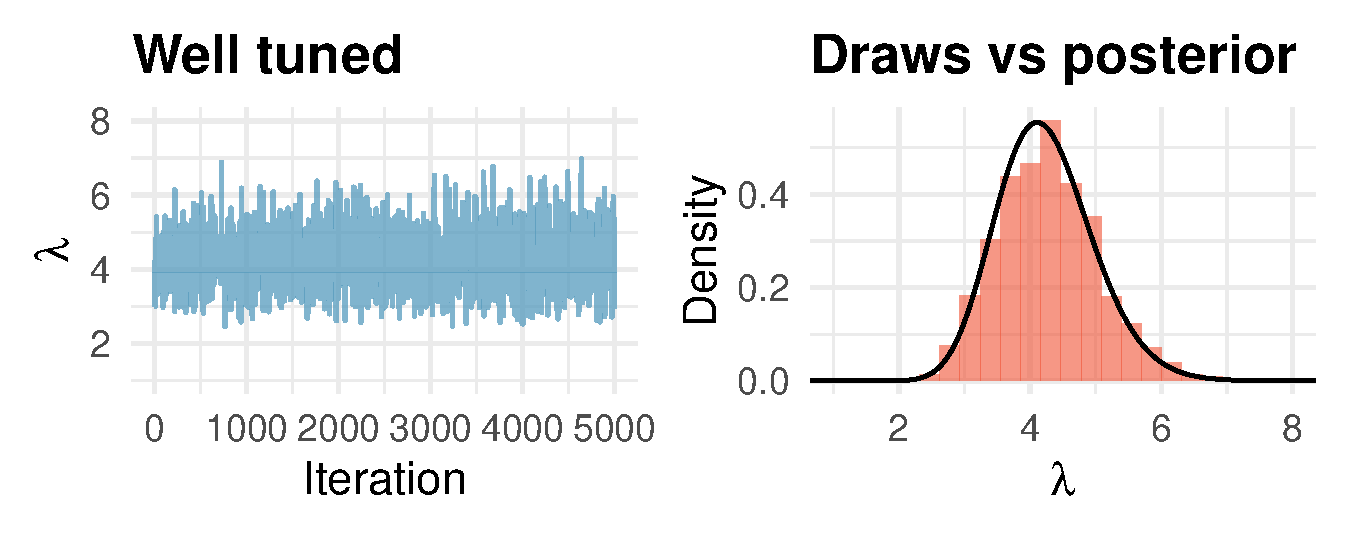
\includegraphics[width=0.94\textwidth]{mcmc_trace_good.pdf}
\end{center}

\vspace{-0.3em}
A well-tuned chain (acceptance $\approx 0.40$) looks like a \hl{fuzzy caterpillar}: noisy fluctuation around the center, no drift, no long flat stretches. Its histogram matches the grid posterior.

\end{frame}

%%%%%%%%%%%%%%%%%%%%%%%%%%%%%%%%%%%%%%%%%%%%%%%%%%%%%%%%%%%%%%%%%%%%%%%%
\begin{frame}
\frametitle{Burn-in: forgetting where you started}

The chain has to start \emph{somewhere}, and that starting value is arbitrary, usually out in the tails.

\pause
\medskip

\keyidea{The first stretch of the chain is still influenced by its arbitrary start and is not yet drawing from the posterior. Discard it: that discarded stretch is the \hl{burn-in}. Read it off the trace plot and keep only the part after the chain has settled into its steady band.}

\pause
\medskip

A few hundred iterations is typical here. Everything we report (mean, interval, $P(\lambda > 3)$) uses only the \hl{post-burn-in} draws.

\end{frame}

%%%%%%%%%%%%%%%%%%%%%%%%%%%%%%%%%%%%%%%%%%%%%%%%%%%%%%%%%%%%%%%%%%%%%%%%
\begin{frame}[fragile]
\frametitle{A sick chain: step too small}
\examplehead{Whale sightings}

\begin{center}
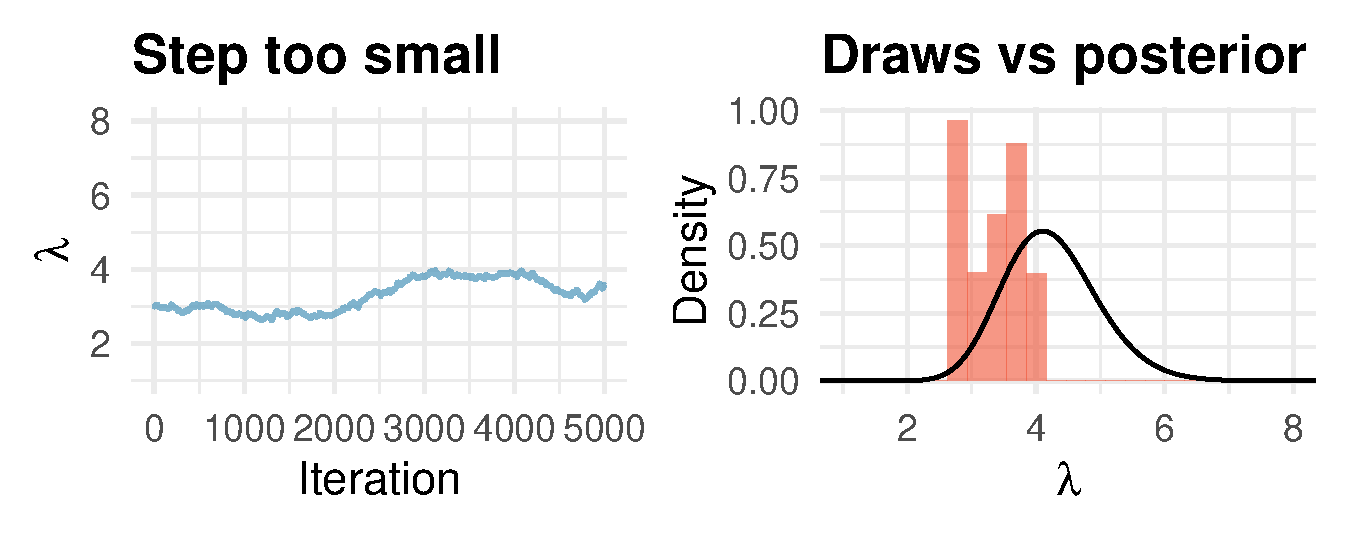
\includegraphics[width=0.94\textwidth]{mcmc_trace_small.pdf}
\end{center}

\vspace{-0.3em}
Step $0.01$: acceptance $\approx 0.99$, but each move is tiny, so the chain \hl{crawls} and never explores the whole posterior in 5{,}000 steps. The histogram is lopsided: the tails were never reached.

\end{frame}

%%%%%%%%%%%%%%%%%%%%%%%%%%%%%%%%%%%%%%%%%%%%%%%%%%%%%%%%%%%%%%%%%%%%%%%%
\begin{frame}[fragile]
\frametitle{A sick chain: step too large}
\examplehead{Whale sightings}

\begin{center}
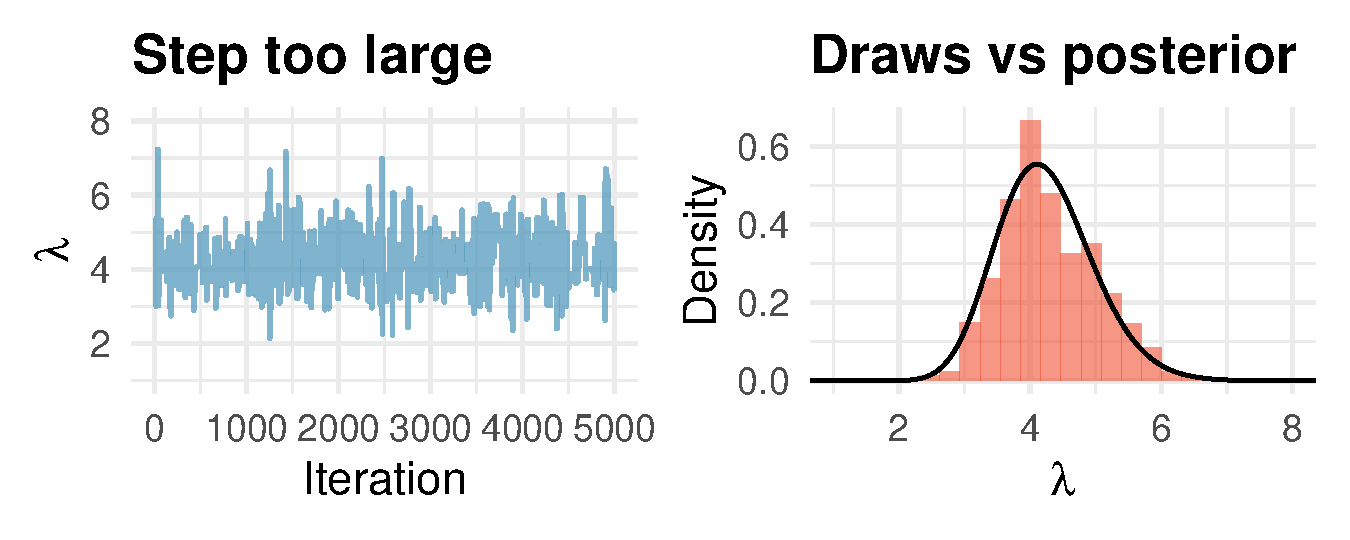
\includegraphics[width=0.82\textwidth]{mcmc_trace_large.pdf}
\end{center}

\vspace{-0.7em}
Step $8.0$: acceptance $\approx 0.11$, so the chain \hl{sticks}.

\dq{Acceptance was $0.99$, $0.40$, $0.11$. Which would you flag from that alone?}

\end{frame}

%%%%%%%%%%%%%%%%%%%%%%%%%%%%%%%%%%%%%%%%%%%%%%%%%%%%%%%%%%%%%%%%%%%%%%%%
\begin{frame}
\frametitle{Three numbers that say ``trust it''}

A trace plot shows gross problems; these three numbers show subtle ones. Software reports all three, so you only need to know what each measures:

\medskip
\begin{itemize}
    \item \hl{$\widehat{R}$:} run \emph{several} chains from different starts; if they agree, $\widehat{R} \approx 1$. Above ${\sim}1.01$ $\Rightarrow$ \textbf{not converged}.
    \pause
    \item \hl{ESS:} draws are \emph{correlated}, so 5{,}000 of them are worth fewer independent draws. ESS is that equivalent count, and you want it in the hundreds.
    \pause
    \item \hl{MCSE:} how much your reported mean would wobble on a re-run. About (posterior SD)$/\sqrt{\text{ESS}}$, so drawing more shrinks it.
\end{itemize}

\end{frame}

%%%%%%%%%%%%%%%%%%%%%%%%%%%%%%%%%%%%%%%%%%%%%%%%%%%%%%%%%%%%%%%%%%%%%%%%
\begin{frame}
\frametitle{From algorithms to software}

You will never code RWMH by hand in practice, but knowing what is under the hood tells you what the diagnostics mean.

\medskip
\begin{itemize}
    \item RWMH is the simplest \hl{Metropolis--Hastings} algorithm. Smarter variants (\hl{HMC}, Hamiltonian Monte Carlo, and \hl{NUTS}, the No-U-Turn Sampler) use the posterior's shape to propose better moves, but keep the same accept/reject logic.
    \pause
    \medskip
    \item \hl{Probabilistic programming} tools (Stan, PyMC, \ldots): you write down the model, the software runs the sampler and returns posterior draws, plus $\widehat{R}$, ESS, and MCSE automatically.
    \pause
    \medskip
    \item Your job shifts from \emph{doing} the sampling to \emph{judging} it: always read the trace and those three numbers before trusting a result.
\end{itemize}
\end{frame}

%%%%%%%%%%%%%%%%%%%%%%%%%%%%%%%%%%%%%%%%%%%%%%%%%%%%%%%%%%%%%%%%%%%%%%%%
\section{Wrap-up}

%%%%%%%%%%%%%%%%%%%%%%%%%%%%%%%%%%%%%%%%%%%%%%%%%%%%%%%%%%%%%%%%%%%%%%%%
\begin{frame}
\frametitle{Summary}

\begin{itemize}
\item Non-conjugate models have \hl{no formula} for the normalizing constant, so we \hl{approximate} the posterior rather than solve for it.
\pause
\item \hl{Grid:} evaluate prior $\times$ likelihood on a grid and normalize, so the integral becomes a sum. Fine in a few dimensions; the grid explodes as parameters multiply.
\pause
\item \hl{MCMC:} propose, accept-or-reject by the density ratio, repeat. The chain visits each $\lambda$ in proportion to the posterior, so the draws \emph{are} a sample. Scales to many dimensions.
\pause
\item \hl{Tune and diagnose:} acceptance $\sim$20--50\%, discard \hl{burn-in}, read the \hl{trace plot}, check \hl{$\widehat{R}$, ESS, MCSE}.
\end{itemize}

\end{frame}

%%%%%%%%%%%%%%%%%%%%%%%%%%%%%%%%%%%%%%%%%%%%%%%%%%%%%%%%%%%%%%%%%%%%%%%%
\begin{frame}
\frametitle{Coming up next}

\hl{We can now get a posterior for any model}, conjugate or not, one parameter or many. That was the last missing piece of machinery.

\vspace{0.4em}
\begin{itemize}
\item \hl{Lecture 20: posterior inference and prediction.} With posterior draws in hand, we \emph{use} them. \hl{Credible intervals} and \hl{hypothesis tests} (deferred from Lectures 18 and 19), \hl{model comparison}, and \hl{prediction} for new data (BR!\ Ch.\ 8).
\pause
\item And \hl{predictive checking}: simulate fake data from the fitted model and ask whether it looks like the data you actually saw, a direct test of whether the model is any good.
\end{itemize}

\end{frame}

%%%%%%%%%%%%%%%%%%%%%%%%%%%%%%%%%%%%%%%%%%%%%%%%%%%%%%%%%%%%%%%%%%%%%%%%
% Activity Frame
%%%%%%%%%%%%%%%%%%%%%%%%%%%%%%%%%%%%
\begin{frame}
\frametitle{In-class activity}

You'll work in \textbf{pairs} (one analyst, one guide).

\medskip
\begin{itemize}
\item Pick up the worksheet.
\item Work through the problems together.
\item \hl{Don't use Gen AI except for debugging}
\item Your worksheet will be collected and graded.
\end{itemize}

\medskip
\textbf{Recommendations:}
\begin{itemize}
\item Read each question carefully before starting the code.
\item Discuss your answers with your partner before writing them down.
\end{itemize}

\end{frame}


\end{document}

